\chapter{Background}\label{C:backgroundsurvey}
\section{Rule Extraction}

A survey in 1995 focuses on rule extraction algorithms \cite{andrews1995survey}, identifying the reasons for needing these algorithms along with introducing ways to categorise and compare them. Motivation behind scientific study is always crucial so why is understanding the knowledge contained inside Artificial Neural Networks's (ANN's) important? The key points identified are that the ANN might of discovered some rule or patten in the data which is currently not known, being able to extract these rules would give humans a greater understanding of the problem. Another, perhaps more significant reason is the application of ANN's to systems which can effect the safety of human lives, i.e. Aeroplanes, Cars. If using an ANN in the context of a system involving human safety it is important to be certain of the knowledge inside the ANN, to ensure that the ANN wont take any dangerous actions.\\

There are three categories that rule extraction algorithms fall into \cite{andrews1995survey}. An algorithm in the \textbf{decompositional} category focuses on extracting rules from each hidden/output unit. If an algorithm is in the \textbf{pedagogical} category then rule extraction is thought of as a learning process, the ANN is treated as a black box and the algorithm learns a relationship between the input and output vectors. The third category, \textbf{electic}, is a combination of decompositional and pedagogical. Electic accounts for algorithms which inspect the hidden/output neurons individually but extracts rules which represent the ANN globally \cite{tickle1998truth}.\\

To further divide the categories two more classifications are introduced. One measures the portability of rule extraction techniques, i.e. how easily can they be applied to different types of ANN's. The second is criteria to assess the quality of the extracted rules, these are accuracy, fidelity, consistency, comprehensibility \cite{andrews1995survey}.

\begin{enumerate}
\item A rule set is \textbf{Accurate} if it can generalize, i.e. classify previously unseen examples.
\item The behaviour of a rule set with a high \textbf{fedelity} is close to that of the ANN it was extracted from.
\item A rule set is \textbf{consistent} if when trained under different conditions it generates rules which assign the same classifications to unseen examples.
\item The measure of \textbf{comprehensibility} is defined by the number of rules in the set and the number of literals per rule.
\end{enumerate}

One rule extraction algorithm presented in 2000 by Tsukimoto is able to extract boolean rules from ANNs in which neurons have monotonically increasing activations, such as the sigmoid function \cite{tsukimoto2000extracting}. The algorithm can be applied to problems with boolean or continuous inputs however only the boolean case will be considered here.\\

Each neuron is written as a boolean operation on its inputs, this is done in the following manner. Consider a neuron $m$ in an MLPN with $n$ inputs, construct a truth table, T, with $n$ inputs. Let $f_i (i \in [0, 2^n])$ represent the activation of $m$ when given row $i$ as input and define $r_i = \land_{j=1}^{n} l_j$, the conjunction of all literals in the row $i$ in T, e.g. if $n=2$ then for row $(1,0)$ $r_i = x_1 \land \lnot x_2$. The approximation of $m$ is given by 

\begin{align}
	\lor_{i=1}^{2^n}\ g_i \land r_i
\end{align}

where $g_i$ is given by

\[
g_i =
\begin{cases}
1 & \text{if $f_i \geq \frac{1}{2}$} \\
0 & \text{if $f_i < \frac{1}{2}$} \\
\end{cases}
\]

By starting with the first hidden layer and progressing through the network an expression for the network can be extracted. Figure \ref{alg:rule-extraction-tsukimoto} shows an algorithm for extracting rules from an MLPN.

\begin{figure}[H]
\begin{lstlisting}[mathescape=true]
function extractRulesMLPN(network)
  prev_expressions = network.inputs
  for layer in network
    expressions = {}
    patters = all input patters for layer
    for each neuron (n) in layer
      exp = And(Or({literals(p), $p \in $patterns n(p) > $\frac{1}{2}$}))
      expressions.add(substitute prev_expressions into exp)
	  
    prev_expressions = expressions
\end{lstlisting}
	\caption{Rule Extraction Algorithm presented in \cite{tsukimoto2000extracting}}
	\label{alg:rule-extraction-tsukimoto}
\end{figure}

The algorithm presented in figure \ref{alg:rule-extraction-tsukimoto} is certainly exponential time in terms of $n$, a polynomial time algorithm is also presented but deriving such an algorithm is beyond the scope of this report.\\

\section{Noisy Neurons} \label{sec:background-noisy-neurons}
MLPNs are universal function approximators and as such can achieve a high accuracy across a broad range of problems. There are many equivelent weight representations of an MLPN which give the same solutions, this makes interpreting the network difficult \cite{LearningLogicalActivations}. By restricting the possible relationships between a neurons inputs and outputs the problem intepretation becomes easier. The two functions OR and AND make intuative sense which is a good reason to pick them over other possible options.\\
 
In 2016 the concept of Noisy-OR and Noisy-AND neurons where described \cite{LearningLogicalActivations}. Noisy neurons are derived from the Noisy-OR relation\cite{LearningLogicalActivations}, developed by Judea Pearl \cite{russell1995modern}, a concept in Bayesian Networks. A Bayesian Network represents the conditional dependencies between random variables in the form of a directed acyclic graph.

\begin{figure}[H]
	\centering
	\begin{minipage}[b]{0.4\textwidth}
		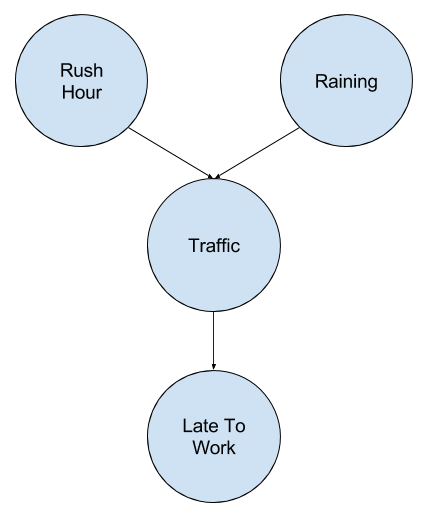
\includegraphics[width=\textwidth]{bayesian-network-example.png}
		\caption{}
		\label{fig:bayesian-network-example}
	\end{minipage}
	\hfill
\end{figure}

Figure \ref{fig:bayesian-network-example} is a Bayesian network, it demonstrates the dependency between random variables "Rush Hour", "Raining", "Traffic", "Late To Work". The connections show dependencies i.e. Traffic influences whether you are late to work, and it being rush hour or raining influences whether there is traffic.\\

Consider a Bayesian Network having the following configuration, take some node $D$ with $S_1,..., S_n$ as parents i.e. $S_i$ influences the node $D$, each $S_i$ is independent from all others. The relationship between D and its parents is if $S_1\ OR\ ...\ OR\ S_n$ is true then $D$ is true. Let $\epsilon_i$ be the uncertainty that $S_i$ influence $D$ then $P(D = 1| S_1 = 1, , S_n = 1)$ can be defined.

\begin{align}
P(D = 1 | S_1 = 1, ..., S_n = 1) = 1 - \prod^n_{i=1} \epsilon_i
\label{equ:noisy-or-relation}
\end{align}

Equation \ref{equ:noisy-or-relation} shows the noisy or relation \cite{LearningLogicalActivations}. In the context of a neuron, the inputs $x_1, ..., x_n$ represent the probability that inputs $1, ..., n$ are true. Consider the output of a neuron as conditionally dependent on the inputs, in terms of a Bayesian Network each $x_i$ is a parent of the neuron. Each $\epsilon_i$ is the uncertainty as to whether $x_i$ influences the output of the neuron. How can weights and inputs be combined to create a final activation value for the neuron. First consider a function $f(\epsilon, x)$ which computes the irrelevance of input x. Some conditions that can be placed on $f$ are given in \cite{LearningLogicalActivations}. (1) $\epsilon = 1$ means that $f(\epsilon, x) = 1$, (2) $x = 1$ means that $f(\epsilon, x) = 1$, (3) Monotonically increasing in $\epsilon$ and decreasing in x. Let $f(x, \epsilon) = \epsilon^x$. The definitions for Noisy-OR and Noisy-AND gates can now be given.

\begin{definition}
	A \textbf{Noisy-OR} Neuron has weights $\epsilon_1, ..., \epsilon_n \in (0,1]$ which represent the irrelevance of corresponding inputs $x_1, ..., x_n \in [0,1]$. The activation of a Noisy-OR Neurons is.
	
	\begin{align}
	a = 1 - \prod^p_{i=1} (\epsilon_i^{x_i}) \cdot \epsilon_b
	\label{equ:noisy-or-activation-1}
	\end{align}
\end{definition}

\begin{definition}
	A \textbf{Noisy-AND} Neuron has weights $\epsilon_1, ..., \epsilon_n \in (0, 1]$ which represent the irrelevance of corresponding inputs $x_1, ..., x_n \in [0,1]$. The activation of a Noisy-AND Neurons is.
	
	\begin{align}
	a = \prod^p_{i=1} (\epsilon_i^{1 - x_i}) \cdot \epsilon_b
	\label{equ:noisy-and-activation-1}
	\end{align}
\end{definition}

Both these parametrisations reduce to discrete logic gates when there is no noise, i.e. $\epsilon_i = 0$ for all $i$.\\

\section{Logical Neural Networks}
ANN's containing of Noisy-OR and Noisy-AND neurons are called Logical Neural Networks (LNN's), if the network consists of only Noisy neurons then it a pure LNN. LNN's have been applied to the MINST dataset with promising results. Experiments with different combinations of logical and standard (sigmoid, soft-max) neurons have shown that pure LNN's where able to achieve an error of 8.67\%, where a standard perceptron/softmax network was able to achieve an error of 3.13\%. This reduction in performance does not come without reward, the pure LNN yields a simpler (sparser) and more interpretable network \cite{LearningLogicalActivations}. Training LNN's which are not pure have been shown to have reduced performance (compared to standard ANN's) and no interpretability benefit.\\

\section{CNF \& DNF}
A boolean formula is in Conjunctive Normal Form (CNF) if and only if it is a conjunction (and) of clauses. A clause in a CNF formula is given by a disjunction (or ) of literals. A literal is either an atom or the negation of an atom, an atom is one of the variables in the formula.\\

Consider the boolean formula $\lnot a \lor (b \land c)$, the CNF is $(\lnot a \lor b) \land (\lnot a \lor c)$. In this CNF formula the clauses are $(\lnot a \lor b)$, $(\lnot a \lor c)$, the literals used are $\lnot a$, $b$, $c$ and the atoms are $a$, $b$, $c$.\\

A boolean formula is in Disjunctive Normal Form (DNF) if and only if it is a disjunction (or) of clauses. A DNF clause is a conjunction (and) of literals. Literals and atoms are defined the same as in CNF formulas.\\

Consider the boolean formula $\lnot a \land (b \lor c)$, the DNF is $(\lnot a \land b) \lor (\lnot a \land c)$.\\

\subsection{CNF \& DNF from Truth Table} \label{subsec:construct-cnfdnf}
Given a truth table representing a boolean formula, constructing a DNF formula involves taking all rows which correspond to True and combining them with an OR operation. To construct a CNF one combines the negation of any row which corresponds to False by an OR operation and negates it.

\begin{theorem}
	The maximum number of clauses in a CNF or DNF formula is $2^n$
	\label{thm:max-clause-cnfdnf}
\end{theorem}

\begin{proof}
	Assume the goal is to find the CNF and DNF for a Boolean formula B of size $n$, for which the complete truth table is given. The truth table has exactly $2^n$ rows.\\
	
	First assume a CNF is being constructed, this is achieved by taking the OR of the negation of all rows corresponding to False, the NOT operation leaves the number of clauses unchanged. At most there can be $2^n$ rows corresponding to False, consequently there are at most $2^n$ clauses in the CNF.\\
	
	A similar argument shows that the same holds for DNF.
\end{proof}

\section{Logical Normal Form Networks}
In 1996 a class of networks, called Logical Normal Form Networks (LNFNs), where developed \cite{herrmann1996backpropagation}, focusing on learning the underlying CNF or DNF for a boolean expression which describes the problem. The approach relies on a specific network configuration along with restriction the function space of each neuron, allowing them to only perform an OR or AND on a subset of their inputs, such OR and AND neurons are called Disjunctive and Conjunctive retrospectively. If the trained network is able to achieve a low enough accuracy then rules can be extracted from the network in terms of a Boolean CNF or DNF expression \cite{herrmann1996backpropagation}.\\

The algorithm which extracts rules from LNFNs would be Electic and certainly is not Portable as the algorithm is specific to the LNFN architecture. It is not possible to further classify the rule extraction algorithm as the research developing it lacks any experimental results, much justification is also missing making the LNFNs difficult to reproduce.\\


